\documentclass[12pt,a4paper]{article}

\usepackage{iftex}
\ifPDFTeX
    \usepackage[utf8]{inputenc}
    \usepackage[T5]{fontenc}
    \usepackage[vietnamese]{babel}
    \usepackage{lmodern}
\else
    \usepackage{fontspec}
    \setmainfont{Times New Roman}
\fi
\usepackage{geometry}
\usepackage{longtable}
\usepackage{booktabs}
\usepackage{array}
\usepackage{enumitem}
\usepackage{hyperref}
\usepackage[table]{xcolor}
\usepackage{listings}
\usepackage{amsmath}
\usepackage{graphicx}
\usepackage{float}

\geometry{margin=2.5cm}
\hypersetup{
    colorlinks=true,
    linkcolor=blue,
    urlcolor=blue,
    citecolor=blue
}

\lstset{
    basicstyle=\ttfamily\small,
    breaklines=true,
    frame=single,
    columns=fullflexible
}

% ── Trình bày bảng rõ ràng: tô màu xen kẽ từng dòng + giãn dòng + viền hàng tiêu đề ──
\definecolor{rowalt}{gray}{0.90}      % màu nền dòng xen kẽ
\definecolor{headbg}{gray}{0.80}      % màu nền dòng tiêu đề
\renewcommand{\arraystretch}{1.35}    % tăng chiều cao dòng cho dễ đọc

\title{Báo cáo biện minh lựa chọn thiết kế dựa trên lý thuyết Özsu và Valduriez}
\author{Project: Distributed Watermark Tracker / Log Delay Compensator}
\date{}

\begin{document}

% Bật tô màu xen kẽ cho mọi bảng phía sau (dòng tiêu đề giữ trắng, thân bảng xen kẽ xám nhạt)
\rowcolors{2}{white}{rowalt}

\maketitle

\section{Mục đích báo cáo}

Báo cáo này biện minh các lựa chọn thiết kế chính của dự án dựa trên lý thuyết hệ cơ sở dữ liệu phân tán của Özsu và Valduriez. Dự án không phải là một hệ quản trị cơ sở dữ liệu quan hệ phân tán truyền thống, nhưng vẫn có các bài toán cốt lõi của \textit{Distributed Data Management}: dữ liệu được chia thành các \textit{partitions}, xử lý bởi nhiều \textit{nodes}, điều phối bằng \textit{global metadata}, nhân bản để tăng \textit{availability}, phục hồi sau lỗi, và được trình bày cho người dùng như một hệ thống xử lý logic thống nhất.

Báo cáo dựa trên các đặc tả thiết kế và kiến trúc triển khai thực tế của hệ thống xử lý dòng dữ liệu watermark logic phân tán.

Dự án có hai hướng thiết kế chính:

\begin{enumerate}
    \item \textbf{Strict Watermark}: ưu tiên \textit{correctness}, \textit{consistency}, \textit{Exactly-Once Processing} và không mất dữ liệu do \textit{late arrival}.
    \item \textbf{Heuristic Watermark}: ưu tiên \textit{low latency}, \textit{site autonomy}, ước lượng thích nghi bằng \textit{DDSketch}, và xử lý dữ liệu muộn thông qua \textit{DLQ} cùng \textit{correction}.
\end{enumerate}

Hai thiết kế đều tuân theo các nguyên tắc của hệ cơ sở dữ liệu phân tán, nhưng chọn hai điểm đánh đổi khác nhau giữa \textit{consistency}, \textit{availability}, \textit{latency}, \textit{autonomy} và \textit{communication cost}.

\section{Cơ sở lý thuyết Özsu và Valduriez}

Theo Özsu và Valduriez, thiết kế một hệ cơ sở dữ liệu phân tán cần được đánh giá qua các khía cạnh sau:

\begin{longtable}{p{0.25\textwidth} p{0.34\textwidth} p{0.33\textwidth}}
\toprule
\textbf{Khái niệm lý thuyết} & \textbf{Ý nghĩa trong Distributed Database} & \textbf{Ánh xạ trong dự án} \\
\midrule
\endhead
\textbf{Fragmentation / Partitioning} & Chia dữ liệu thành các mảnh để mỗi \textit{site} xử lý một phần dữ liệu toàn cục. & \textit{Kafka partitions} chia luồng log vô hạn cho nhiều \textit{Workers}. \\
\textbf{Allocation} & Quyết định mảnh dữ liệu được lưu và xử lý ở đâu. & \textit{Partitions} được gán cho \textit{Worker nodes}; khi lỗi có thể \textit{reassign}. \\
\textbf{Replication} & Lưu nhiều bản sao dữ liệu hoặc metadata để tăng \textit{availability} và khả năng phục hồi. & \textit{Kafka replication}, \textit{Coordinator HA}, \textit{Aggregator HA}, \textit{checkpoints}, \textit{Tier 2/Tier 3 state}. \\
\textbf{Distributed Processing} & Thực thi xử lý trên nhiều \textit{sites} và hợp nhất kết quả cục bộ. & \textit{Workers} xử lý \textit{local windows/local watermarks}; \textit{Coordinator/Aggregator} tính \textit{global watermark}. \\
\textbf{Distributed Coordination} & Điều phối trạng thái hoặc metadata dùng chung giữa nhiều \textit{sites}. & \textit{Coordinator} tính \texttt{W\_global}; \textit{Aggregator} tính \texttt{W\_global\_h}. \\
\textbf{Consistency Management} & Đảm bảo tính đúng khi nhiều node cùng cập nhật trạng thái logic. & \textit{Exactly-Once}, \textit{Fencing Token}, \textit{Failback State Machine}, \textit{Idempotent Output}. \\
\textbf{Reliability and Recovery} & Phục hồi khi có lỗi node, storage hoặc communication. & \textit{Checkpoint}, \textit{Replay}, \textit{DLQ}, \textit{Tiered State Storage}, \textit{Disaster Recovery}. \\
\textbf{Transparency} & Che giấu sự phân tán để người dùng nhìn thấy một hệ thống logic thống nhất. & Người dùng nhìn thấy một pipeline xử lý log thống nhất dù bên dưới có nhiều nodes và partitions. \\
\textbf{Communication Cost} & Tối ưu chi phí truyền thông giữa các node. & \textit{Strict Watermark} chấp nhận cost cao hơn; \textit{Heuristic Watermark} giảm \textit{blocking coordination}. \\
\textbf{Site Autonomy} & Cho phép mỗi site hoạt động cục bộ khi có thể. & \textit{Heuristic Workers} tự ước lượng watermark bằng \textit{DDSketch}. \\
\bottomrule
\end{longtable}

Những khái niệm này là cơ sở để biện minh hai hướng thiết kế của dự án.

\section{Bảng ký hiệu và biến của dự án (Glossary)}

Bảng dưới đây tổng hợp các ký hiệu toán học và biến trạng thái được sử dụng xuyên suốt báo cáo, làm tham chiếu cho các công thức ở các mục biện minh thiết kế phía sau:

\begin{longtable}{p{0.20\textwidth} p{0.56\textwidth} p{0.16\textwidth}}
\toprule
\textbf{Ký hiệu} & \textbf{Ý nghĩa} & \textbf{Giá trị / Phạm vi} \\
\midrule
\endhead
$T_{event}$ & Mốc thời gian logic (event-time) khi sự kiện được sinh ra tại nguồn. & giây \\
$T_{arrival}$ & Mốc thời gian vật lý khi Worker tiếp nhận sự kiện. & giây \\
$\ell$ & Độ trễ truyền dẫn của bản ghi: $\ell = T_{arrival} - T_{event}$. & giây \\
\texttt{[window\_start, window\_end]} & Khoảng Tumbling Window định danh một cửa sổ tổng hợp. & 5 s \\
$P_k$ & Phân mảnh (partition) Kafka thứ $k$. & $k \in [0, 11]$ \\
$LW_i(P_k)$ & Watermark cục bộ của Worker $i$ cho phân mảnh $P_k$ (chế độ Strict). & giây \\
$W_{global}$ & Watermark toàn cục Strict: $\min$ các $LW_i$ trên phân mảnh active. & giây \\
$W_{h,i}^{P_k}$ & Watermark thích ứng cục bộ (Heuristic) của Worker $i$ cho $P_k$. & giây \\
$W_{global\_h}$ & Watermark toàn cục Heuristic: $\min$ các $W_{h,i}^{P_k}$. & giây \\
$T_{event\_max}$ & Event-time lớn nhất quan sát được trên một phân mảnh. & giây \\
$L_{eff}$ & Độ trễ hiệu dụng (lag effective): phân vị $p$ của phân phối $\ell$. & giây \\
$Q_p,\ p$ & Hàm phân vị (quantile) và phân vị mục tiêu để tính $L_{eff}$. & $p \in \{0.99,\, 0.999\}$ \\
$\delta$ (\texttt{DELTA\_BASE\_S}) & Biên an toàn (Wait Time) cố định của chế độ Strict. & 10 s (mặc định) \\
$\alpha$ & Sai số tương đối (relative error) của DDSketch. & 0.01 \\
$\gamma$ & Hệ số log-scale bucket của DDSketch: $\gamma = (1+\alpha)/(1-\alpha)$. & $\approx 1.0202$ \\
$\varepsilon$ & Ngân sách hao hụt (loss budget) của Heuristic: $\varepsilon = 1 - p$. & $\le 1\%$ \\
$term$ & Nhiệm kỳ (Raft term) gắn vào Fencing Token để chống Split-brain. & số nguyên \\
\texttt{IDLE\_TIMEOUT\_S} & Ngưỡng thời gian đánh dấu phân mảnh nhàn rỗi tường minh (\texttt{TEMPORARY\_IDLE}). & 2.0 s \\
\texttt{HEARTBEAT\_TIMEOUT\_S} & Ngưỡng hết hạn nhịp tim để Coordinator xác nhận Worker lỗi. & 10 s \\
\bottomrule
\caption{Bảng ký hiệu và biến trạng thái của hệ thống Distributed Watermark Tracker.}
\label{tab:glossary}
\end{longtable}

\section{Biện minh thiết kế Strict Watermark}

\subsection{Mục tiêu thiết kế}

\textit{Strict Watermark} ưu tiên tính đúng. Một \textit{window} chỉ được emit khi hệ thống có đủ bằng chứng rằng mọi \textit{partitions} liên quan đã đi qua mốc thời gian của window đó.

Mục tiêu chính:

\begin{itemize}
    \item 0\% mất dữ liệu do \textit{late arrival}.
    \item \textit{Exactly-Once Input Processing}.
    \item \textit{Exactly-Once} hoặc \textit{Idempotent Output}.
    \item Phục hồi mạnh khi \textit{Worker}, \textit{Coordinator} hoặc storage gặp lỗi.
    \item \textit{High Availability} thông qua \textit{Coordinator HA} và \textit{Tiered State Storage}.
\end{itemize}

Thiết kế này phù hợp với các nghiệp vụ không chấp nhận sai lệch như \textit{audit logs}, \textit{billing}, \textit{compliance reporting} hoặc \textit{security monitoring}.

\subsection{Lý do thiết kế Strict Watermark trước và Ảnh hưởng của bài toán Straggler}

Trong thiết kế hệ thống xử lý dữ liệu phân tán, việc ưu tiên hiện thực hóa giải pháp \textit{Strict Watermark} trước tiên là một quyết định mang tính chiến lược vì các lý do sau:

\begin{enumerate}
    \item \textbf{Mẫu tham chiếu tính đúng đắn (Correctness Baseline)}: Để đánh giá hiệu quả của bất kỳ giải pháp tối ưu hóa hoặc xấp xỉ nào (như Heuristic), hệ thống cần một mốc so sánh chuẩn xác tuyệt đối (baseline). Strict Watermark cung cấp tính nhất quán mạnh mẽ (Strong Consistency) và bảo đảm dữ liệu hoàn thiện 100\%, đóng vai trò là cột mốc để đo lường mức độ đánh đổi (trade-off) về cả độ trễ và độ hao hụt dữ liệu của Heuristic.
    \item \textbf{Cam kết an toàn tuyệt đối (Safety Guarantees)}: Các nghiệp vụ cốt lõi như đối soát tài chính hay kiểm toán bảo mật đòi hỏi độ chính xác không sai lệch. Bằng cách thiết kế Strict trước, chúng tôi chứng minh rằng hệ thống có khả năng đạt được trạng thái an toàn tối đa trước khi tìm cách hạ thấp tiêu chuẩn để tăng hiệu năng.
    \item \textbf{Xây dựng nền tảng hạ tầng chịu lỗi (Infrastructure Foundation)}: Giải thuật Strict đòi hỏi sự vận hành đồng bộ của các thành phần hạ tầng phức tạp: điều phối phân mảnh ngang, chuyển giao trạng thái Exactly-Once qua 5 bước failback, và bầu chọn đồng thuận qua Raft. Thiết kế Strict trước giúp kiểm thử và hoàn thiện toàn bộ hạ tầng điều phối này một cách độc lập trước khi tích hợp thêm các mô hình thống kê phức tạp.
\end{enumerate}

\paragraph{Bài toán Straggler (Nút cổ chai trạm chậm) và Giải pháp hiện thực hóa:}
Trong lý thuyết xử lý luồng phân tán, giải pháp \textit{Strict Watermark} tiêu chuẩn thường dễ bị tổn thương bởi hiện tượng Straggler (một phân mảnh bị trễ hoặc dừng luồng dữ liệu nạp khiến watermark toàn cục bị nghẽn). Tuy nhiên, thiết kế hệ thống của chúng tôi đã chủ động giải quyết bài toán Straggler trong chế độ Strict bằng hai cơ chế phối hợp:
\begin{itemize}
    \item \textbf{Cơ chế Bỏ qua phân mảnh nhàn rỗi (Idleness Bypass / Bypass Idle Partitions)}: Khi một phân mảnh tạm thời không phát sinh dữ liệu mới vượt quá cấu hình giới hạn thời gian (\texttt{IDLE\_TIMEOUT\_S}), Worker sẽ tự động đánh dấu phân mảnh đó là nhàn rỗi (\texttt{TEMPORARY\_IDLE}) và báo cáo trong heartbeat. Coordinator Leader khi nhận được nhịp tim sẽ tự động loại trừ phân mảnh nhàn rỗi này ra khỏi hàm tối thiểu toàn cục:
    \begin{equation}
        W_{global} = \min_{P_k \notin \text{Idle}} LW_i(P_k)
    \end{equation}
    Điều này cho phép dòng chảy thời gian của toàn cụm tiếp tục tịnh tiến, giải phóng trạng thái cửa sổ của các phân mảnh đang hoạt động bình thường mà không bị nghẽn bởi phân mảnh nhàn rỗi. Khi phân mảnh nhàn rỗi có log mới nạp vào, nó sẽ tự động được đưa trở lại danh sách tính toán watermark toàn cục.
    \item \textbf{Tái phân bổ động dựa trên hết hạn nhịp tim (Heartbeat Timeout Failover)}: Nếu một Worker bị sập vật lý hoặc bị phân mảnh mạng nghiêm trọng (trở thành trạm chậm vĩnh viễn), Coordinator Leader sẽ phát hiện sau khi hết hạn nhịp tim (\texttt{HEARTBEAT\_TIMEOUT\_S} là 10 giây). Hệ thống sẽ kích hoạt giao thức tái phân bổ động, thu hồi quyền sở hữu phân mảnh của node lỗi, tăng \textit{fencing term} logic để phong tỏa các lệnh cũ, và phân phối đều các phân mảnh bị ảnh hưởng cho các Worker còn sống gánh hộ. Worker mới nạp trạng thái từ checkpoint Tier-2 để tiếp tục tiêu thụ dữ liệu, giải phóng nghẽn dòng chảy watermark.
\end{itemize}

Ngược lại, \textit{Heuristic Watermark} tiếp cận giải quyết bài toán Straggler từ góc độ tự trị cục bộ (Site Autonomy): các Worker tự tịnh tiến mốc chốt cửa sổ thích ứng dựa trên quan sát trễ cục bộ (DDSketch). Các bản ghi của các trạm chậm đến sau khi cửa sổ chốt không làm nghẽn hệ thống mà được chuyển hướng sang hàng đợi DLQ để phục vụ việc sửa đổi và đối chiếu đền bù bất đồng bộ sau (Eventual Consistency).

\subsection{Fragmentation và Parallel Processing}

Özsu và Valduriez xem \textit{Fragmentation} là bước thiết kế cốt lõi của hệ phân tán. Dự án áp dụng nguyên tắc này bằng cách chia luồng log thành nhiều \textit{Kafka partitions}.

\begin{longtable}{p{0.42\textwidth} p{0.5\textwidth}}
\toprule
\textbf{Lựa chọn thiết kế} & \textbf{Biện minh theo lý thuyết} \\
\midrule
\endhead
Kafka dùng 12 \textit{partitions}. & Đây là \textit{horizontal fragmentation} của luồng sự kiện. Mỗi partition chứa một phần của luồng log toàn cục. \\
Bốn \textit{Workers} xử lý các nhóm partitions. & Đây là \textit{distributed processing} trên các mảnh dữ liệu, giúp tránh xử lý tập trung tại một node. \\
Mỗi Worker có RocksDB riêng theo partition. & Bảo toàn tính độc lập của mỗi fragment và tránh lock contention giữa partitions. \\
\bottomrule
\end{longtable}

Việc chọn partition làm đơn vị sở hữu là hợp lý vì partition vừa là đơn vị xử lý, vừa là đơn vị phục hồi, \textit{failover} và đảm bảo \textit{Exactly-Once}.

\subsection{Cấp phát và Tái phân bổ động (Allocation \& Reallocation)}

Trong thiết kế cơ sở dữ liệu phân tán, lý thuyết \textit{Allocation} (Cấp phát) quyết định cách đặt các mảnh dữ liệu (fragments) tại các trạm (sites) nhằm tối ưu hóa chi phí truyền thông và cân bằng tải. Dự án áp dụng nguyên lý này bằng cách phân bổ các \textit{Kafka partitions} cố định cho các \textit{Worker nodes} trong điều kiện hoạt động bình thường.

Khi xảy ra sự cố (chẳng hạn như một Worker bị sập), hệ thống áp dụng cơ chế \textbf{Tái phân bổ động có kiểm soát (Controlled Dynamic Reallocation)}:
\begin{itemize}
    \item \textbf{Tái phân bổ cân bằng tải phân tán (Distributed Rebalancing)}: Thay vì dồn toàn bộ các phân mảnh bị ảnh hưởng của node sập cho một node gánh hộ duy nhất (gây ra hiện tượng quá tải cục bộ hoặc nút cổ chai mới), Coordinator Leader sẽ tính toán lại sơ đồ phân mảnh và chia đều chúng cho tất cả các Worker còn sống (ví dụ: chia đều các phân mảnh $P_9, P_{10}, P_{11}$ của Worker 3 cho Worker 0, Worker 1, và Worker 2). Điều này tuân thủ mục tiêu tối ưu hóa hàm phân bổ tải trọng toàn cục của Özsu và Valduriez.
    \item \textbf{Nguyên tắc Độc quyền Sở hữu (Partition Exclusive Ownership)}: Một phân mảnh tại một thời điểm chỉ được xử lý bởi duy nhất một Worker hoạt động. Trạng thái phân mảnh được bảo vệ nghiêm ngặt qua mô hình máy trạng thái (\texttt{ASSIGNED}, \texttt{REASSIGNING}, \texttt{PAUSED}, \texttt{ORPHANED}) lưu trong Raft log, ngăn chặn hoàn toàn việc ghi trùng trạng thái cục bộ lên RocksDB hoặc trùng lặp dữ liệu đầu ra (Idempotent Output).
    \item \textbf{Cơ chế bàn giao failback 5 bước (5-Step Failback State Machine)}: Khi Worker cũ hồi phục và muốn nhận lại phân mảnh, hệ thống thực thi giao thức bàn giao có kiểm soát thông qua các trạng thái gRPC: \texttt{PAUSE} (tạm dừng consume trên node gánh hộ) $\rightarrow$ \texttt{FLUSH\_ACK} (flush trạng thái RocksDB cục bộ xuống Tier-2 Shared Volume, ghi nhận checkpoint offset cuối và gửi phản hồi) $\rightarrow$ \texttt{KAFKA\_REASSIGN} (cập nhật chủ sở hữu mới trong Raft log và cấu hình tiêu thụ) $\rightarrow$ \texttt{SEEK\_RESUME} (Worker hồi phục nạp checkpoint và seek đến offset tiếp theo) $\rightarrow$ \texttt{COMPLETE} (bàn giao hoàn tất, trả về trạng thái hoạt động bình thường). Giao thức này tương đương với mô hình giao tiếp tin cậy trong các hệ quản trị phân tán khi thay đổi cấu hình trạm.
\end{itemize}

Mô hình máy trạng thái phân mảnh (Partition State Machine) bảo vệ nguyên tắc độc quyền sở hữu trong suốt quá trình tái phân bổ:
\begin{figure}[H]
    \centering
    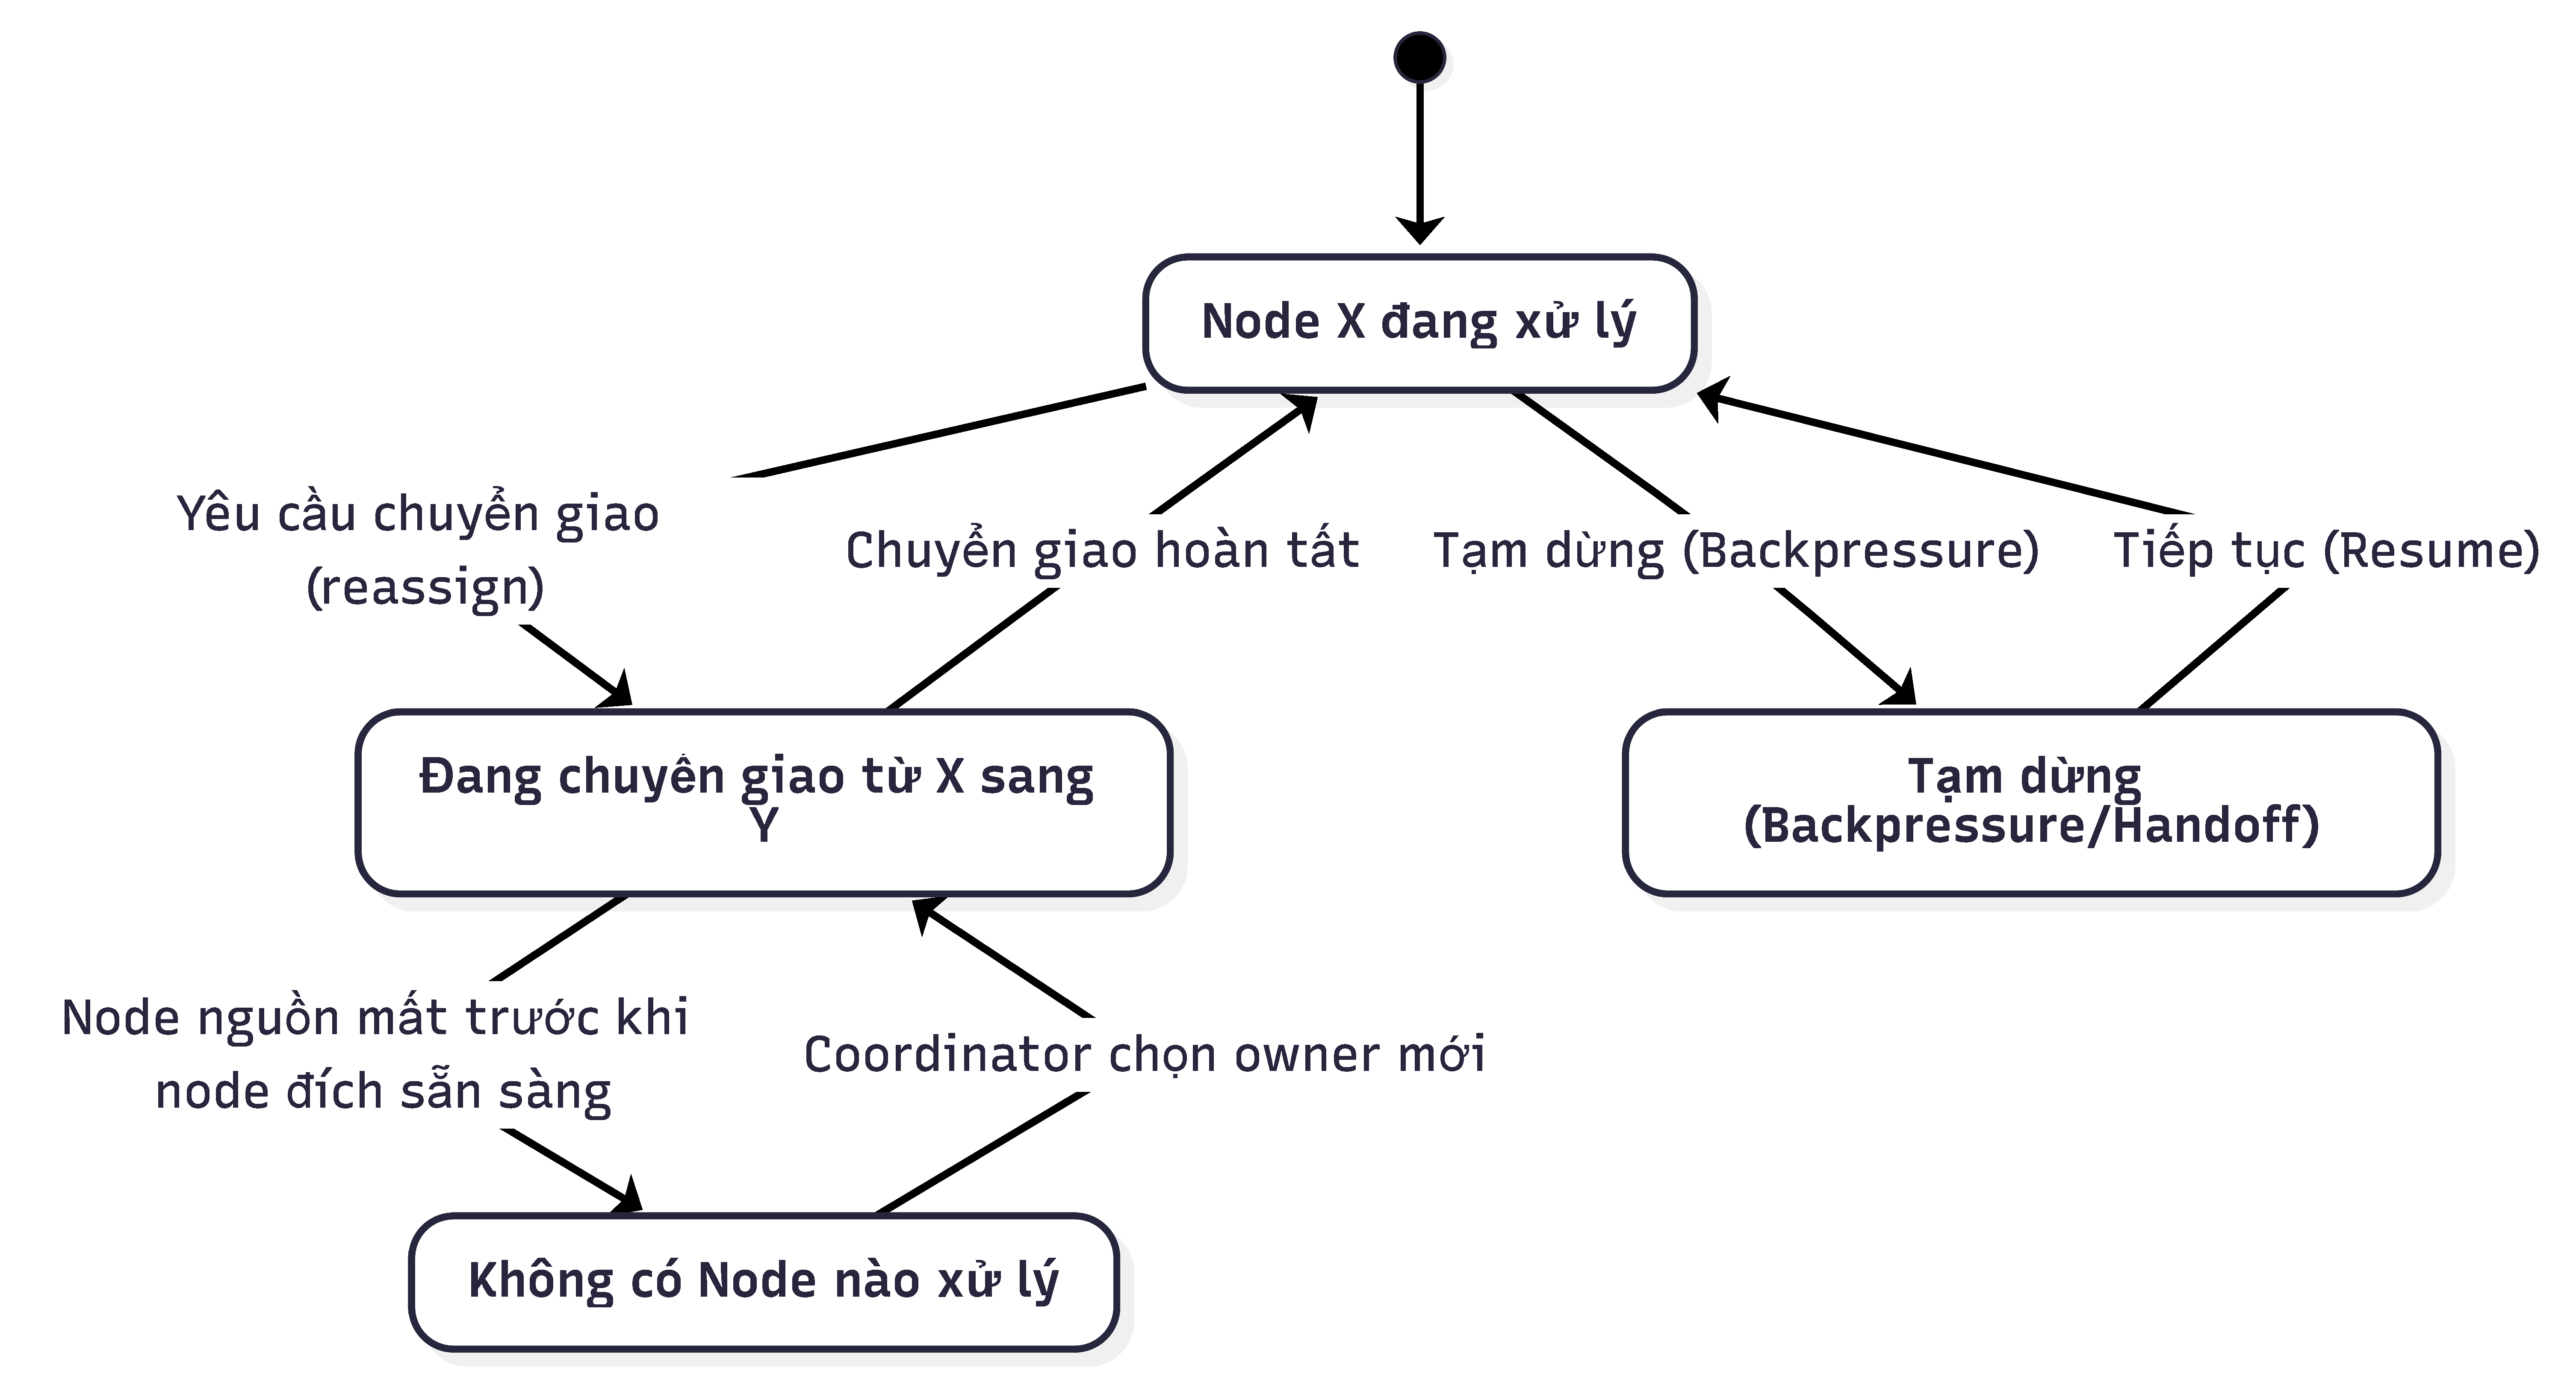
\includegraphics[width=0.85\textwidth,height=6.0cm,keepaspectratio]{Partition State Machine.pdf}
    \caption{Máy trạng thái phân mảnh: \texttt{ASSIGNED} $\to$ \texttt{REASSIGNING} $\to$ \texttt{PAUSED} $\to$ \texttt{ORPHANED}.}
    \label{fig:partitionstatemachine}
\end{figure}

Chuỗi bàn giao failback 5 bước có kiểm soát khi Worker cũ hồi phục và nhận lại phân mảnh:
\begin{figure}[H]
    \centering
    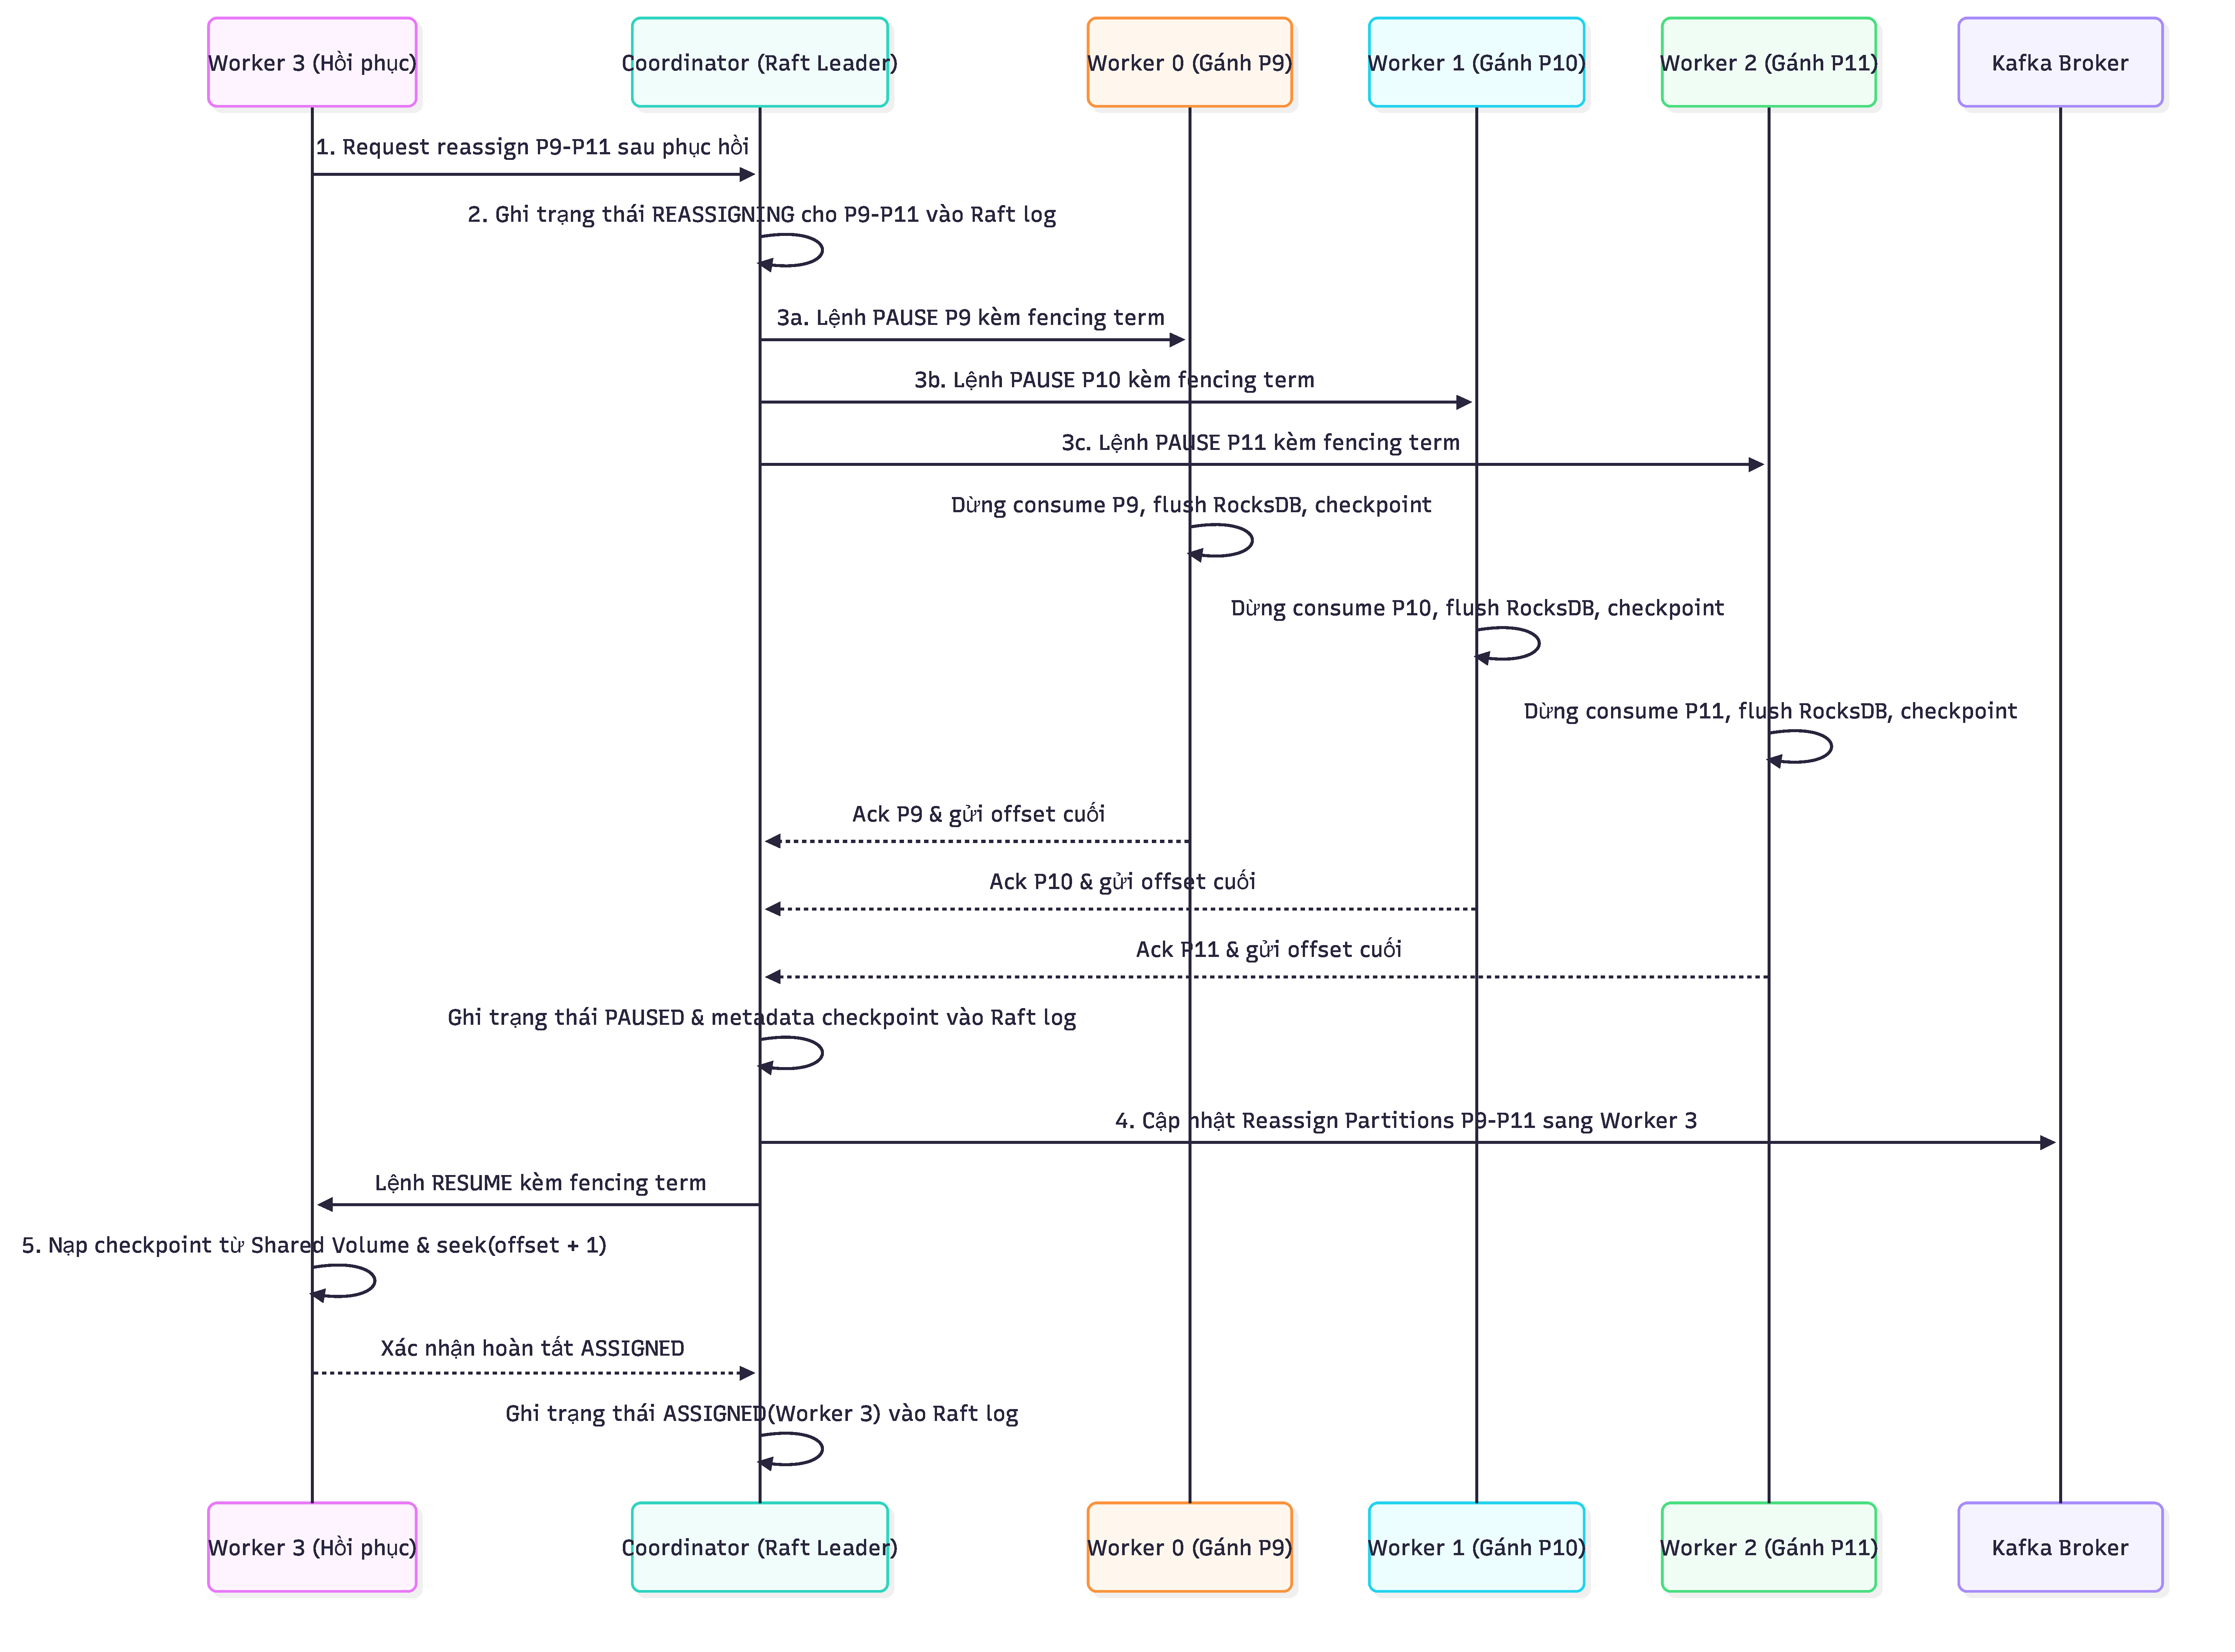
\includegraphics[width=0.9\textwidth,height=8.5cm,keepaspectratio]{5-Step Failback Sequence Diagram.pdf}
    \caption{Sơ đồ trình tự bàn giao Failback 5 bước (PAUSE $\to$ FLUSH\_ACK $\to$ KAFKA\_REASSIGN $\to$ SEEK\_RESUME $\to$ COMPLETE).}
    \label{fig:failbacksequence}
\end{figure}

\subsection{Distributed Coordination và Strong Consistency}

\textit{Strict Watermark} cần một quyết định toàn cục: khi nào một window an toàn để đóng. Mỗi Worker chỉ biết tiến độ cục bộ. Coordinator hợp nhất các \textit{local watermarks}:

\begin{equation}
    W_{global}(t) = \min_{\forall P_k \in \text{Active}} LW_i(P_k)
\end{equation}

Đây là dạng \textit{distributed metadata coordination}. Theo Özsu và Valduriez, khi tính đúng phụ thuộc vào trạng thái của nhiều sites, hệ phân tán cần một cơ chế điều phối metadata toàn cục.

\paragraph{Lựa chọn Cơ chế Đồng thuận (Consensus Selection):}
Để bảo đảm tính nhất quán nghiêm ngặt (Strong Consistency) và chống lỗi phân mảnh mạng (Split-Brain), hệ thống sử dụng hai phương thức đồng thuận khác nhau tùy theo mô hình xử lý:
\begin{itemize}
    \item \textbf{Strict Coordinator (Raft Consensus)}: Được triển khai thông qua cơ chế đồng thuận Raft phân tán. Một nhóm 3 nodes Coordinator chạy thuật toán đồng thuận Raft để bầu chọn Leader và sao chép trạng thái (Leader Election \& State Replication). Mọi thay đổi về phân bổ phân mảnh hay cập nhật watermark toàn cục đều được lưu trữ dưới dạng log đồng thuận được xác nhận bởi đa số (quorum acks). Các Worker sử dụng \textit{Fencing Token/Term} từ Raft để từ chối các chỉ thị lỗi thời từ một Leader cũ bị cô lập mạng.
    \item \textbf{Heuristic Aggregator (ZooKeeper Lock HA)}: Triển khai thông qua cơ chế dự phòng Active-Standby được điều phối qua khóa phân tán của ZooKeeper. Cách tiếp cận này giúp giảm đáng kể chi phí truyền thông (Communication Cost), tăng hiệu năng và hạ thấp độ trễ khi hệ thống không yêu cầu cam kết nhất quán nghiêm ngặt tức thời mà ưu tiên tính tự trị cục bộ (Site Autonomy).
\end{itemize}

\begin{longtable}{p{0.38\textwidth} p{0.52\textwidth}}
\toprule
\textbf{Thành phần Strict} & \textbf{Tương đương trong Distributed Database} \\
\midrule
\endhead
\texttt{LW\_i(P\_k)} & Local site progress metadata. \\
\texttt{W\_global} & Global consistency metadata. \\
Coordinator Leader & Distributed transaction/metadata coordinator. \\
Worker Heartbeat & Site status and progress report. \\
Fencing Token / Term & Cơ chế chống stale coordinator và split-brain. \\
\bottomrule
\end{longtable}

Thiết kế chấp nhận \textit{coordination overhead} vì yêu cầu correctness mạnh hơn yêu cầu latency.

Sơ đồ điều phối Strict: các Worker báo cáo \texttt{LW\_i} qua heartbeat, Coordinator Leader (đồng thuận Raft 3-node) tính \texttt{W\_global} và broadcast ngược lại:
\begin{figure}[H]
    \centering
    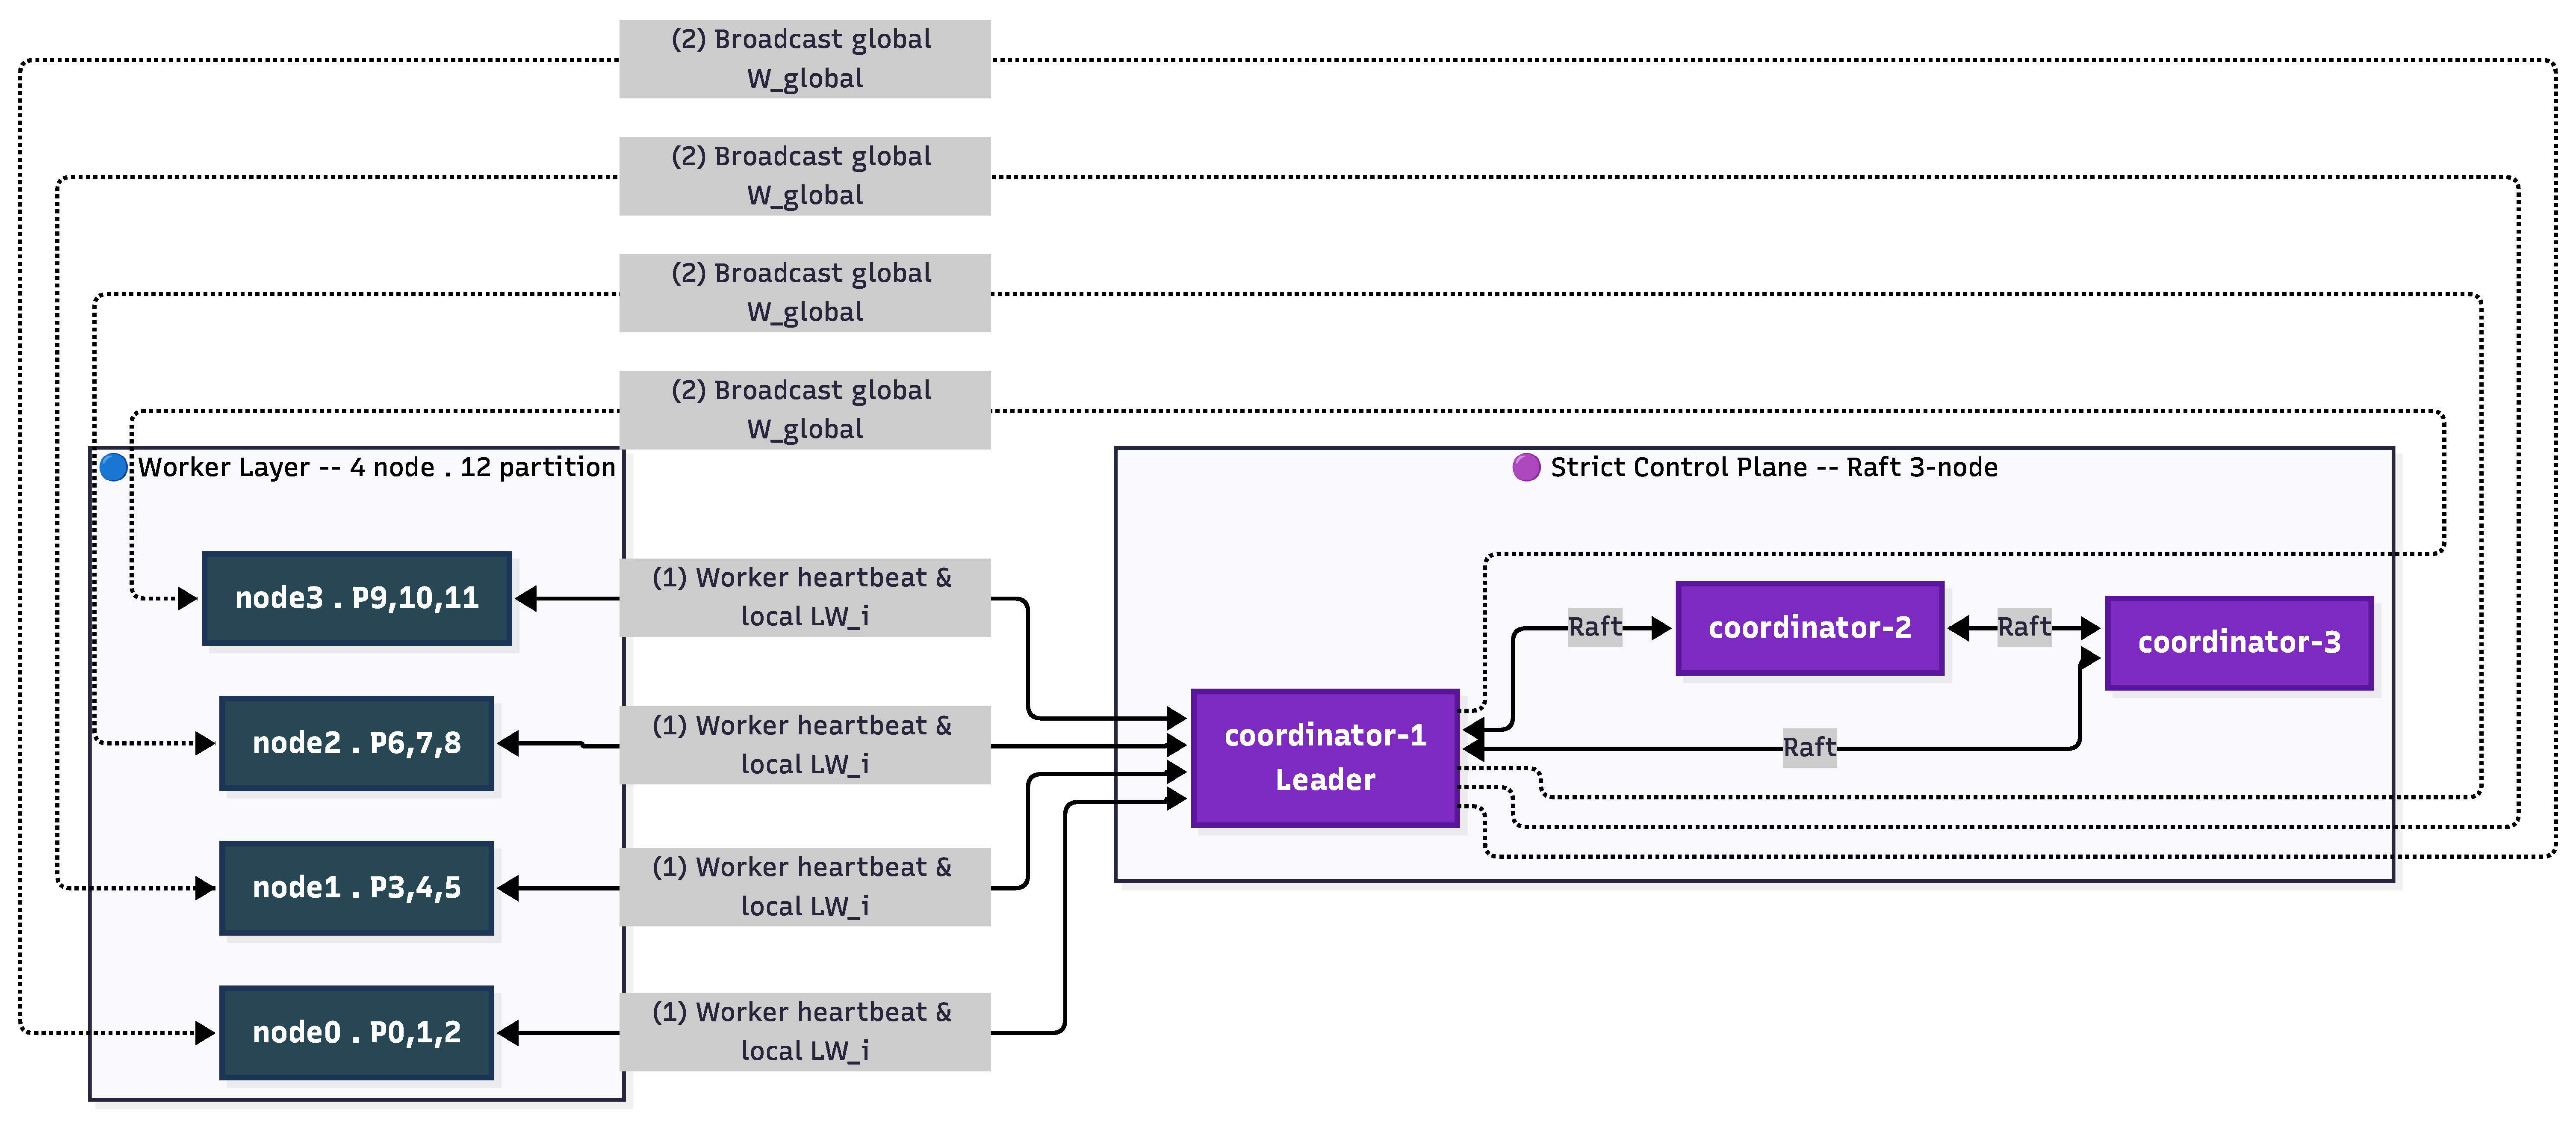
\includegraphics[width=0.9\textwidth,height=7.0cm,keepaspectratio]{domain_4.2.pdf}
    \caption{Luồng điều phối Strict Watermark: hợp nhất \texttt{W\_global = min(LW\_i)} qua cụm Coordinator Raft.}
    \label{fig:strictcoordination}
\end{figure}

\subsection{Punctuation Token như Distributed Progress Metadata}

\textit{Strict Watermark} sử dụng \textit{Punctuation Token} từ upstream để biểu thị rằng một partition đã đi qua một mốc event-time. Ngay cả khi partition idle, hệ thống vẫn phát \textit{Empty Punctuation Token}.

Thiết kế này giải quyết một vấn đề phân tán quan trọng: không có dữ liệu không đồng nghĩa với đã hoàn tất. Nếu không có punctuation, Coordinator không thể phân biệt:

\begin{itemize}
    \item partition thật sự idle,
    \item Ingestor của partition đã lỗi,
    \item partition bị delay do network hoặc broker.
\end{itemize}

Vì vậy, \textit{Punctuation Token} là \textit{progress metadata} rõ ràng, phù hợp với yêu cầu điều phối metadata trong hệ phân tán.

Sơ đồ trình tự xử lý phân mảnh nhàn rỗi bằng Empty Punctuation và Idleness Bypass tường minh:
\begin{figure}[H]
    \centering
    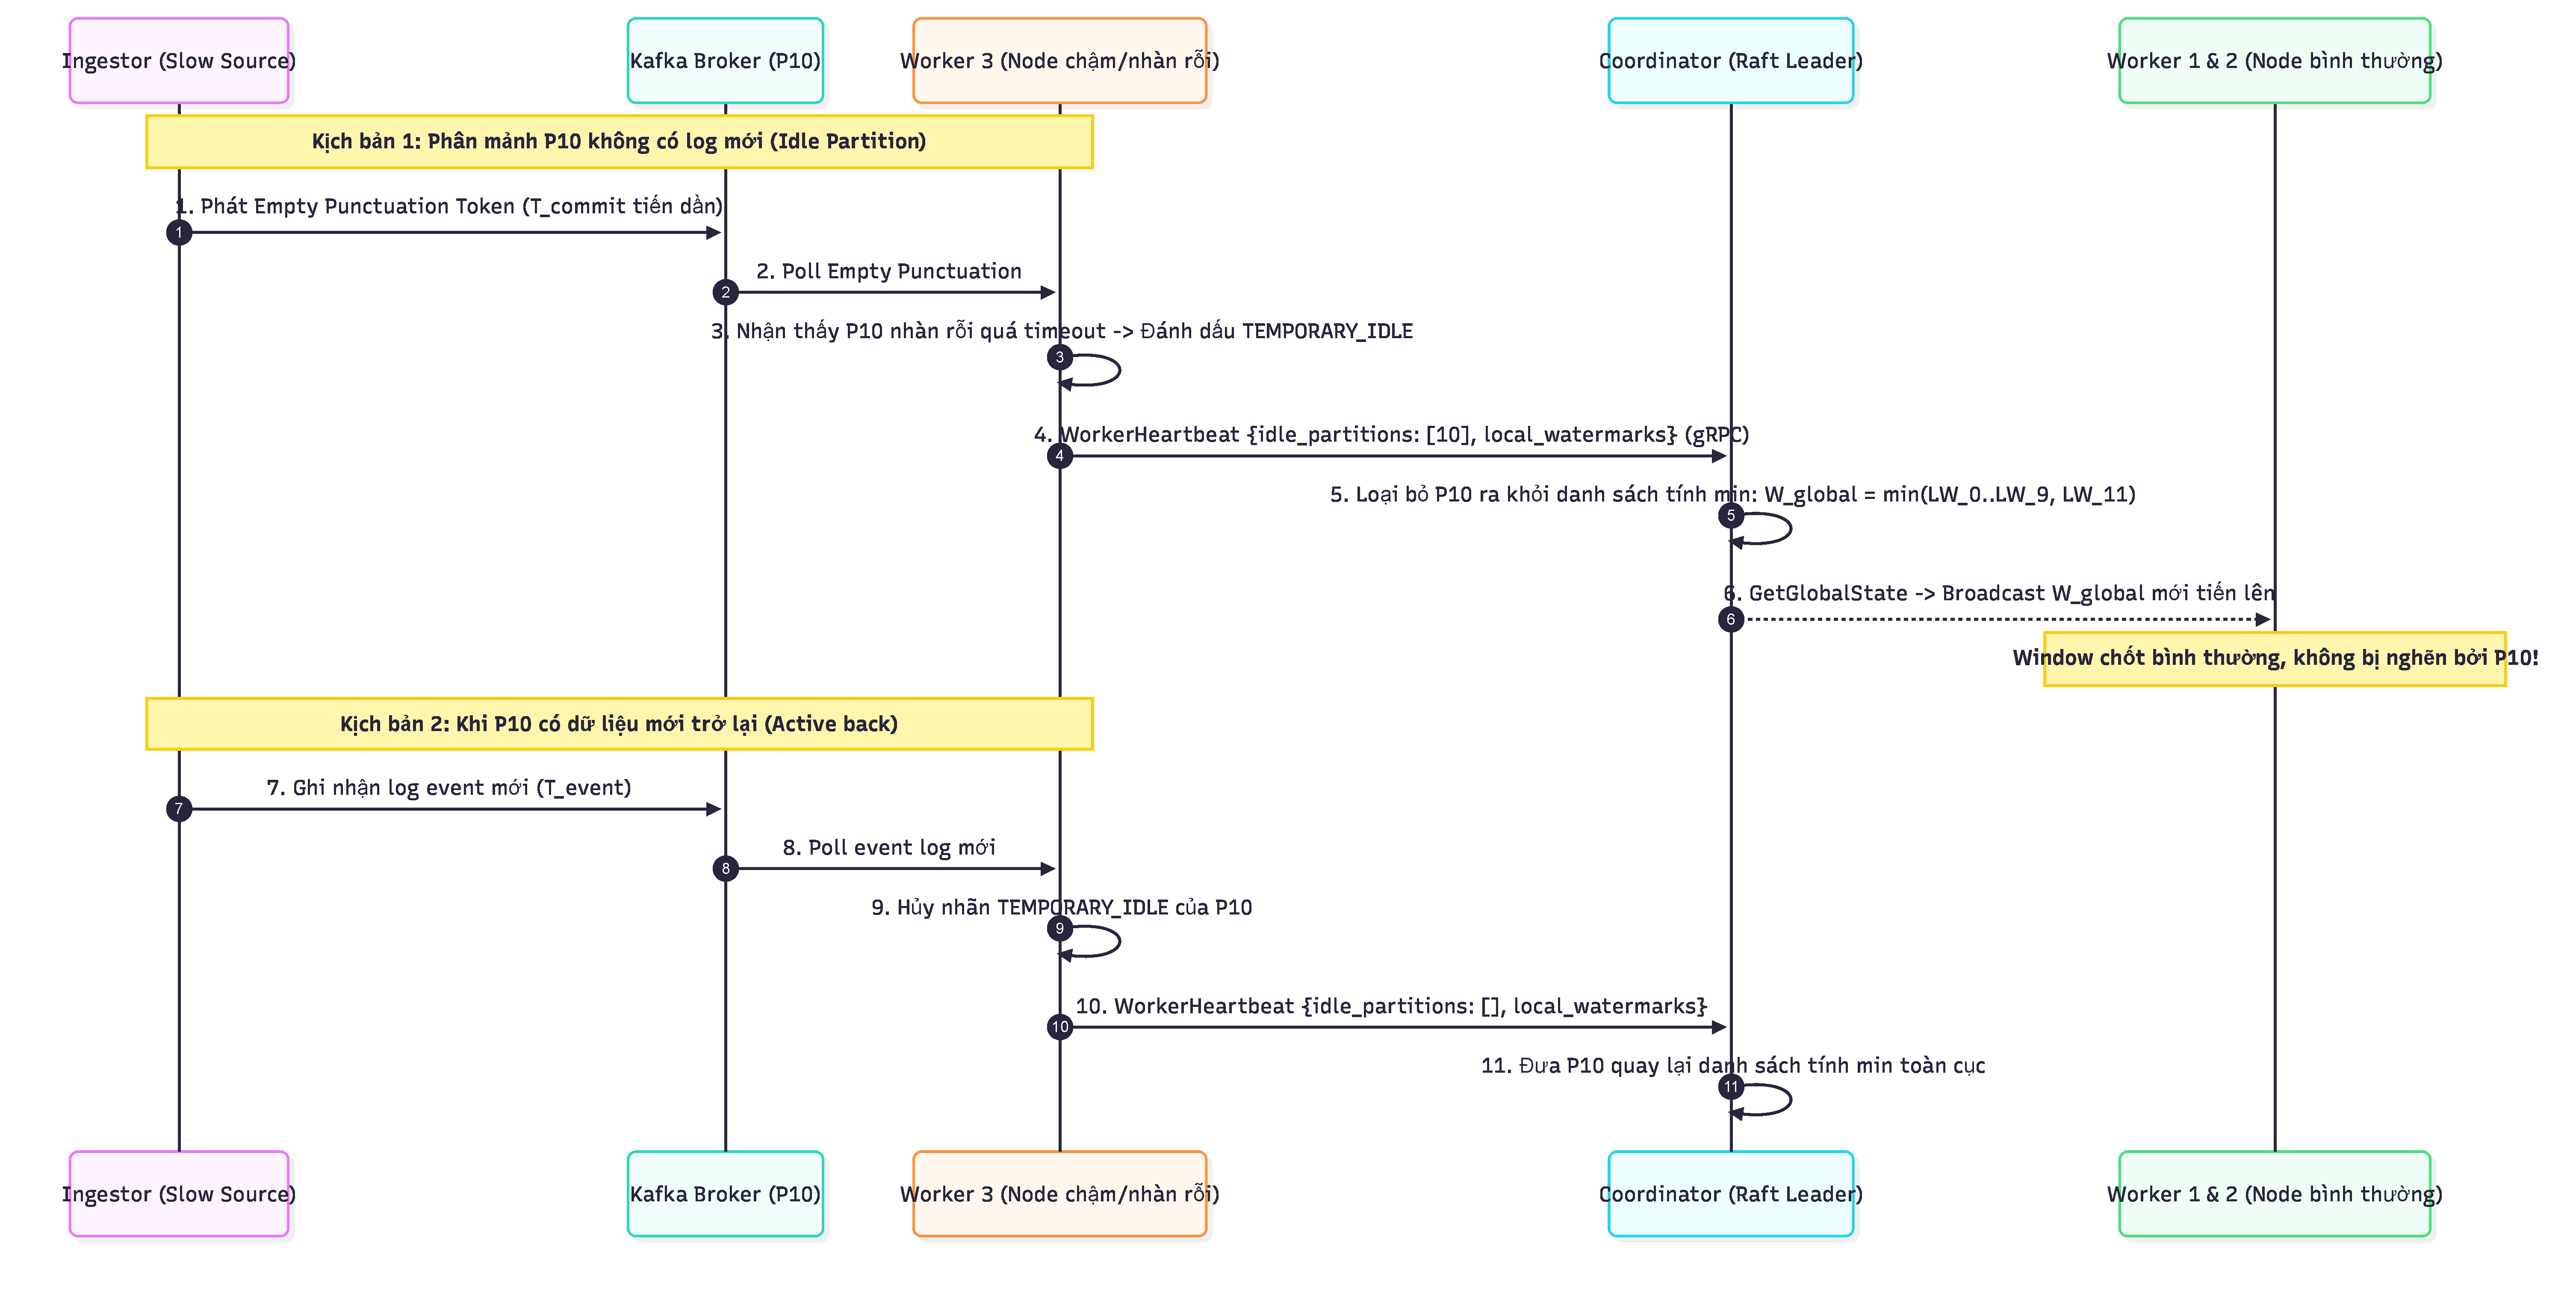
\includegraphics[width=0.9\textwidth,height=8.5cm,keepaspectratio]{Empty Punctuation.pdf}
    \caption{Empty Punctuation giữ \texttt{W\_global} tịnh tiến khi phân mảnh nhàn rỗi, không gây mất dữ liệu khi phân mảnh hoạt động lại.}
    \label{fig:emptypunctuation}
\end{figure}

\subsection{Replication và High Availability}

\textit{Strict Watermark} dùng replication ở nhiều tầng:

\begin{longtable}{p{0.25\textwidth} p{0.35\textwidth} p{0.32\textwidth}}
\toprule
\textbf{Tầng} & \textbf{Cơ chế Replication / Redundancy} & \textbf{Mục đích} \\
\midrule
\endhead
Kafka & Broker replication & Input log bền vững và có thể replay. \\
Coordinator & Raft / ZooKeeper-style HA & Tránh Coordinator single point of failure. \\
State & Tier 2 shared checkpoints & Worker failover nhanh. \\
Disaster Recovery & Tier 3 object storage & Phục hồi khi mất local/shared storage. \\
Output & Transactional hoặc idempotent sink & Tránh duplicate output. \\
\bottomrule
\end{longtable}

Điều này phù hợp với nguyên tắc \textit{Reliability}: dữ liệu và metadata quan trọng phải tồn tại sau lỗi node hoặc lỗi storage.

\subsection{Recovery và Exactly-Once Semantics}

Özsu và Valduriez xem \textit{Recovery} là yêu cầu nền tảng của hệ dữ liệu phân tán. \textit{Strict Watermark} triển khai recovery bằng:

\begin{itemize}
    \item checkpoint \textit{active window state},
    \item lưu Kafka offsets,
    \item replay sau lỗi,
    \item dedup input events,
    \item fencing stale leaders,
    \item đảm bảo mỗi partition chỉ có một owner hợp lệ,
    \item dùng \textit{Exactly-Once} hoặc \textit{Idempotent Output}.
\end{itemize}

\textit{Failback State Machine} đặc biệt quan trọng. Khi Worker đã lỗi quay lại, nó không được tự ý resume partition cũ. Coordinator phải pause owner tạm thời, flush state, ghi checkpoint metadata, chuyển ownership, rồi mới cho Worker phục hồi tiếp tục.

Invariant cốt lõi là:

\begin{equation*}
    \forall\, t,\ \forall\, P_k : \quad \big|\,\mathrm{Owner}(P_k,\, t)\,\big| = 1
\end{equation*}
\begin{center}
    \small\textit{(Bất biến: tại mọi thời điểm, mỗi phân mảnh có đúng một chủ sở hữu xử lý hợp lệ.)}
\end{center}

Invariant này là nền tảng để giữ \textit{Exactly-Once Processing}.

\subsection{Tiered State Storage}

Thiết kế dùng ba tầng lưu trữ:

\begin{longtable}{p{0.25\textwidth} p{0.35\textwidth} p{0.32\textwidth}}
\toprule
\textbf{Tier} & \textbf{Vai trò} & \textbf{Biện minh lý thuyết} \\
\midrule
\endhead
Tier 1: Local RocksDB & Hot state cho active windows. & Data locality và xử lý cục bộ nhanh. \\
Tier 2: Shared Volume & Warm checkpoint cho failover nhanh. & State có thể phục hồi và cấp phát lại. \\
Tier 3: Object Storage & Cold archive và Disaster Recovery. & Reliability dài hạn và storage scalability. \\
\bottomrule
\end{longtable}

Cách tổ chức này phù hợp với nguyên tắc dữ liệu truy cập thường xuyên nên ở gần nơi xử lý, còn bản sao phục hồi phải nằm ngoài node có thể lỗi.

\subsection{Communication Cost Trade-off}

\textit{Strict Watermark} cần:

\begin{itemize}
    \item Worker Heartbeats,
    \item Ingestor Heartbeats,
    \item Punctuation Tokens,
    \item Coordinator Broadcasts,
    \item State Machine Transitions,
    \item Raft/ZooKeeper Coordination.
\end{itemize}

Chi phí truyền thông cao hơn là đánh đổi có chủ đích. Theo Özsu và Valduriez, \textit{Communication Cost} phải được đánh giá cùng với correctness và reliability. Ở đây, hệ thống chọn tăng coordination để đạt \textit{strong consistency} và recovery mạnh.

\subsection{Kết luận cho Strict Watermark}

\textit{Strict Watermark} được biện minh theo lý thuyết Özsu và Valduriez vì nó sử dụng:

\begin{itemize}
    \item \textit{Fragmentation} để mở rộng,
    \item \textit{Allocation/Reallocation} để quản lý partition ownership,
    \item \textit{Replication} để tăng reliability,
    \item \textit{Distributed Coordination} để duy trì global watermark consistency,
    \item \textit{Recovery Protocols} để chịu lỗi,
    \item \textit{Exactly-Once Semantics} để bảo toàn correctness,
    \item \textit{Transparency} để che giấu sự phức tạp phân tán.
\end{itemize}

Thiết kế này phù hợp khi \textit{correctness} quan trọng hơn \textit{low latency}.

\section{Biện minh thiết kế Heuristic Watermark}

\subsection{Mục tiêu thiết kế}

\textit{Heuristic Watermark} ưu tiên \textit{low latency} và khả năng thích nghi. Thiết kế này không chờ \textit{Punctuation Token} nghiêm ngặt từ upstream hoặc \textit{blocking global coordination}. Thay vào đó, Worker dùng \textit{DDSketch} để ước lượng độ trễ và sinh \textit{heuristic watermark}.

Mục tiêu chính:

\begin{itemize}
    \item giảm end-to-end latency,
    \item chấp nhận \textit{bounded loss} hoặc xử lý late data có kiểm soát,
    \item ước lượng watermark thích nghi,
    \item giảm phụ thuộc vào strict upstream signals,
    \item correction dữ liệu muộn thông qua DLQ.
\end{itemize}

Thiết kế này phù hợp với realtime dashboard, monitoring hoặc near-realtime analytics, nơi kết quả nhanh có giá trị hơn việc chờ completeness tuyệt đối.

\subsection{Fragmentation và Distributed Processing}

Tương tự \textit{Strict Watermark}, \textit{Heuristic Watermark} dùng Kafka partitions và nhiều Workers. Đây vẫn là áp dụng nguyên tắc \textit{Fragmentation}.

\begin{longtable}{p{0.42\textwidth} p{0.5\textwidth}}
\toprule
\textbf{Lựa chọn thiết kế} & \textbf{Biện minh lý thuyết} \\
\midrule
\endhead
Kafka partitions chia luồng log. & Horizontal fragmentation giúp xử lý song song. \\
Workers xử lý partitions độc lập. & Distributed processing giảm bottleneck trung tâm. \\
Mỗi Worker ước lượng local lag. & Computation được đẩy về site nơi dữ liệu được quan sát. \\
\bottomrule
\end{longtable}

Điểm khác biệt chính là \textit{Heuristic Watermark} trao nhiều quyền tự trị hơn cho Worker. Worker không cần chờ upstream \textit{Punctuation Token} để ước lượng tiến độ.

\subsection{Site Autonomy}

Özsu và Valduriez xem \textit{Site Autonomy} là một thuộc tính quan trọng của hệ phân tán. \textit{Heuristic Watermark} áp dụng trực tiếp nguyên tắc này:

\begin{itemize}
    \item Mỗi Worker quan sát local arrival delay.
    \item Mỗi Worker cập nhật DDSketch riêng.
    \item Mỗi Worker tính local heuristic watermark \texttt{W\_h\_i\textasciicircum\{P\_k\}}.
    \item Aggregator chỉ hợp nhất local watermarks thành \texttt{W\_global\_h}.
\end{itemize}

Điều này làm giảm vai trò của coordinator trung tâm. Worker có thể tiến triển dựa trên quan sát cục bộ, giúp hệ thống phản hồi nhanh hơn và giảm blocking.

\subsection{DDSketch như Distributed Metadata}

\textit{DDSketch} được dùng để tóm tắt phân phối lag. Đây không phải dữ liệu nghiệp vụ thô mà là metadata về hành vi của stream. Theo góc nhìn distributed database, đây là một compact local summary có thể dùng để ước lượng tiến độ cục bộ.

Lựa chọn DDSketch hợp lý vì:

\begin{itemize}
    \item bounded memory,
    \item cập nhật hiệu quả,
    \item ước lượng quantile,
    \item mergeability,
    \item phù hợp với heavy-tail delay distribution.
\end{itemize}

Hệ thống ước lượng:

\begin{align*}
    \ell    &= T_{arrival} - T_{event}, \\
    L_{eff} &= Q_p(\{\ell\}), \\
    W_h     &= T_{event\_max} - L_{eff}.
\end{align*}

Đây là thiết kế \textit{approximate distributed metadata}: giảm coordination cost nhưng vẫn có cơ sở thống kê để quyết định event-time progress.

\subsection{Aggregator HA và Reduced Coordination}

\textit{Heuristic Watermark} dùng Aggregator nhẹ hơn so với Strict Coordinator. Aggregator theo dõi heuristic watermarks theo partition và tính:

\begin{equation}
    W_{global\_h}(t) = \min_{\forall P_k \in \text{Active}} W_{h,i}^{P_k}(t)
\end{equation}

Cơ chế này vẫn có một điểm hợp nhất toàn cục, nhưng nhẹ hơn:

\begin{itemize}
    \item không yêu cầu upstream punctuation,
    \item không cần strict failback state machine cho mỗi quyết định watermark,
    \item có thể chạy \textit{Active-Standby} bằng ZooKeeper lock,
    \item tập trung vào global progress aggregation thay vì chứng minh strict correctness.
\end{itemize}

Theo Özsu và Valduriez, khi ứng dụng cho phép correction, giảm \textit{blocking coordination} để giảm latency là một trade-off hợp lý.

Sơ đồ điều phối Heuristic: Aggregator (Active-Standby qua khóa ZooKeeper) gom \texttt{W\_h} từ các Worker tự trị mà không chặn dòng xử lý:
\begin{figure}[H]
    \centering
    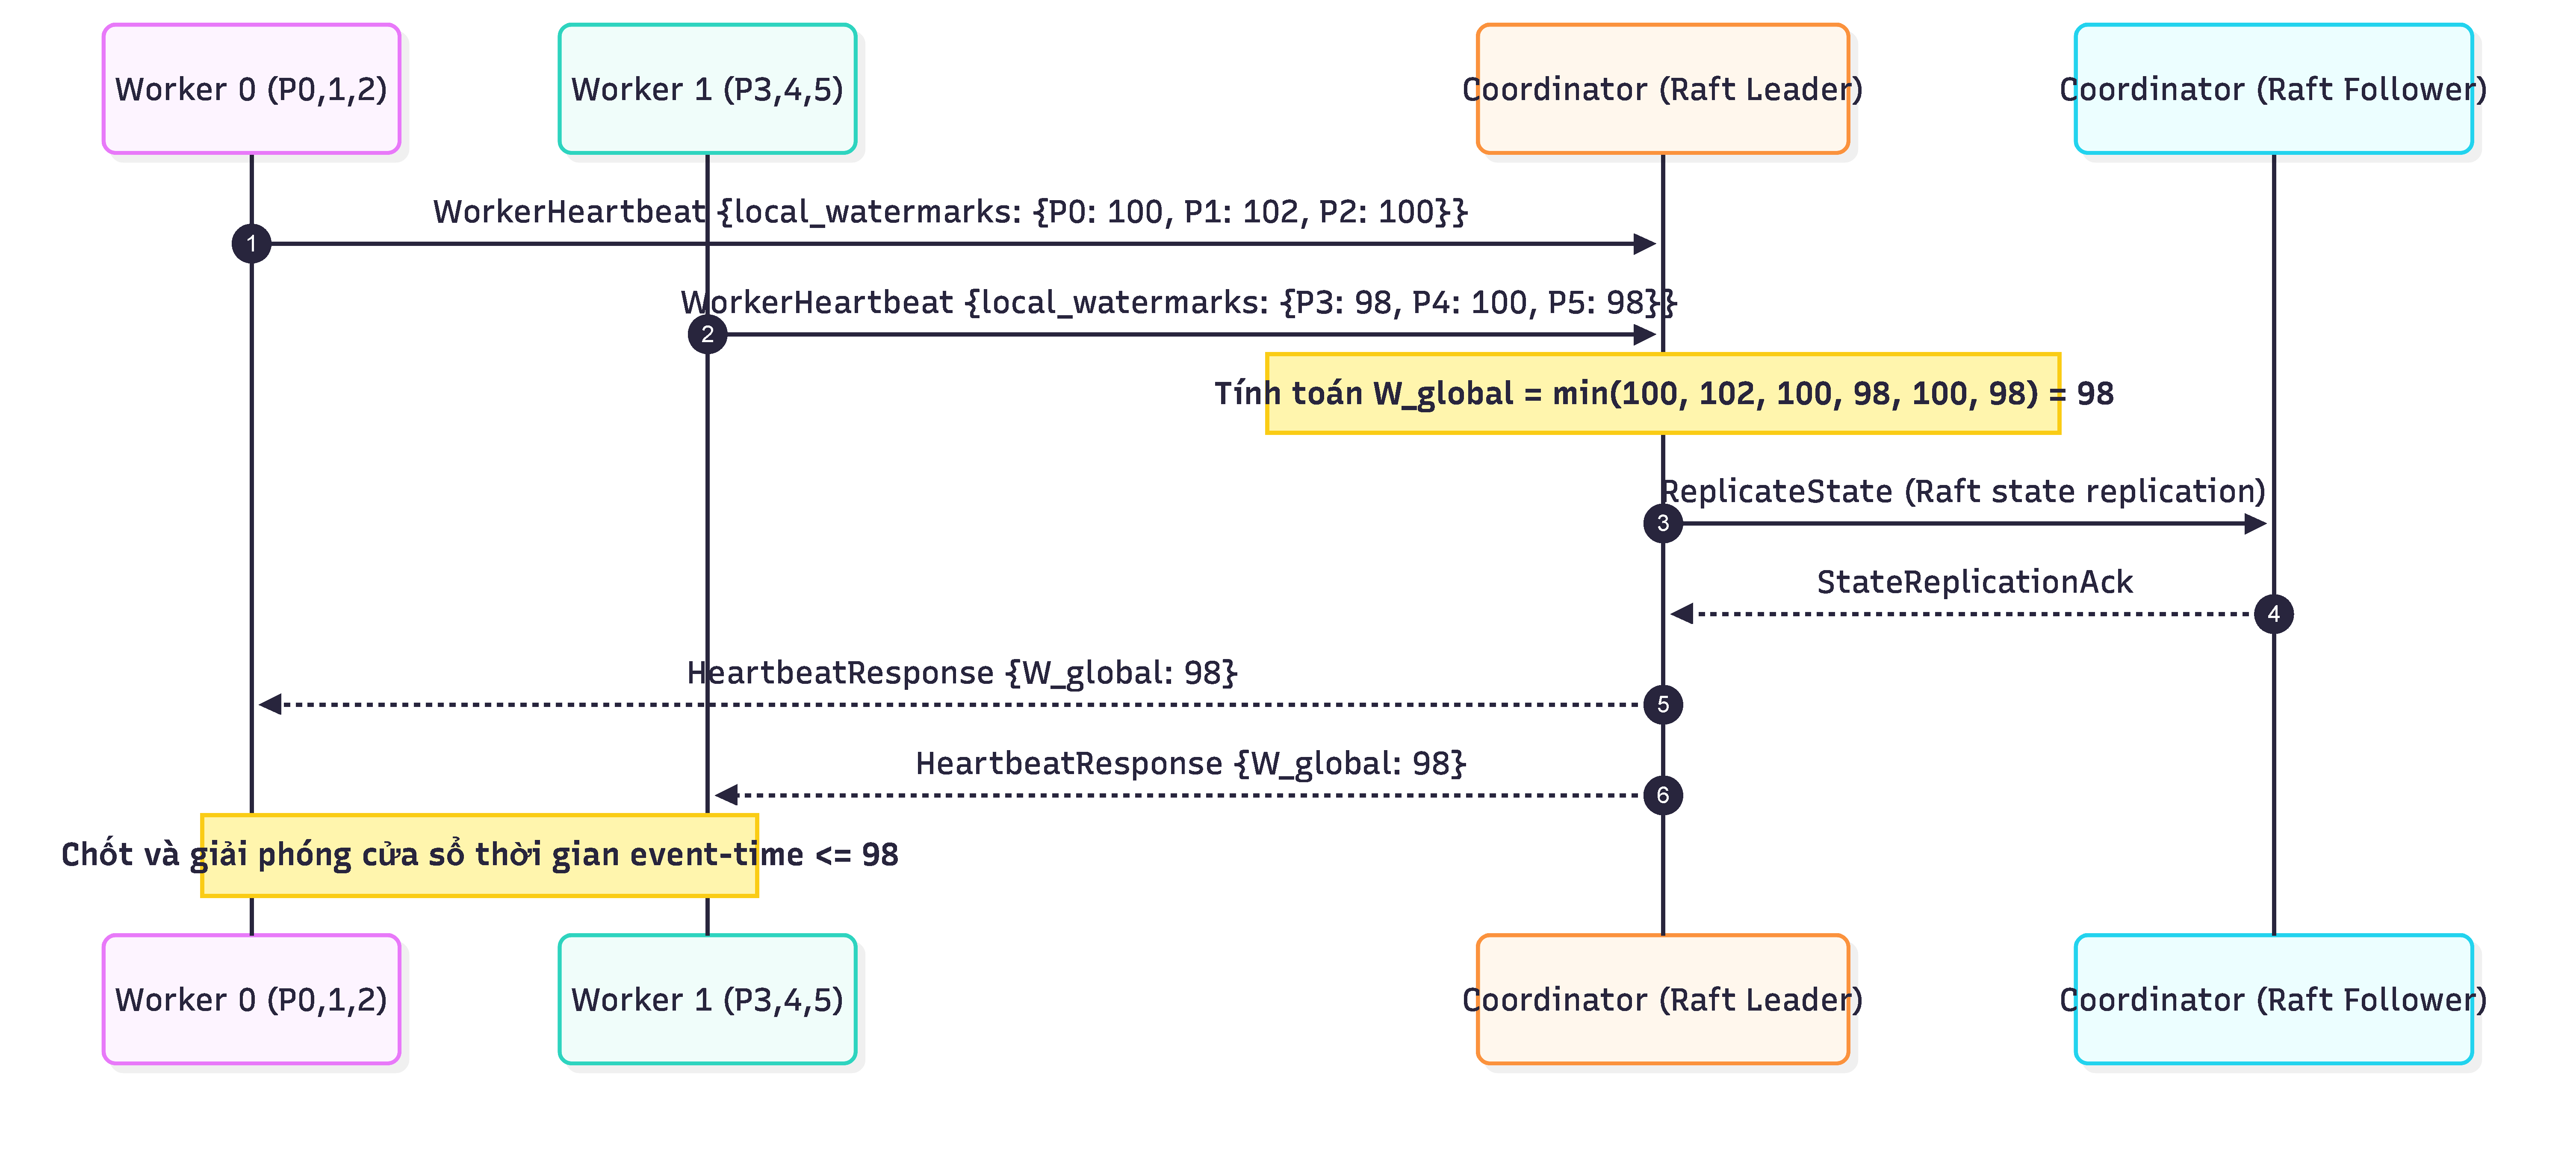
\includegraphics[width=0.9\textwidth,height=7.0cm,keepaspectratio]{Heuristic Aggregator.pdf}
    \caption{Luồng điều phối Heuristic Watermark: Aggregator HA hợp nhất \texttt{W\_global\_h = min(W\_h)} thích ứng.}
    \label{fig:heuraggregation}
\end{figure}

\subsection{Eventual Correction thay cho Immediate Strong Consistency}

\textit{Heuristic Watermark} có thể emit window trước khi toàn bộ late data đến. Điều này làm yếu \textit{immediate consistency}. Thiết kế bù lại bằng:

\begin{itemize}
    \item DLQ cho late logs,
    \item Correction Messages,
    \item Downstream Update Patterns,
    \item Final Reconciliation,
    \item Correction Deduplication.
\end{itemize}

Đây là mô hình gần với \textit{Eventual Consistency} và \textit{Compensating Transaction}. Kết quả ban đầu có thể mang tính speculative, nhưng hệ thống ghi nhận late data và có thể sửa kết quả sau.

\begin{longtable}{p{0.42\textwidth} p{0.5\textwidth}}
\toprule
\textbf{Vấn đề} & \textbf{Giải pháp trong Heuristic Watermark} \\
\midrule
\endhead
Late log đến sau watermark. & Đưa vào DLQ. \\
Window đã emit nhưng thiếu dữ liệu. & Tính Correction Message. \\
Downstream nhận correction trùng. & Dùng Correction Deduplication. \\
Kết quả ban đầu chưa phải final. & Dùng Versioning hoặc Final Reconciliation. \\
\bottomrule
\end{longtable}

Thiết kế không drop dữ liệu âm thầm. Nó chuyển mô hình correctness từ \textit{Immediate Strong Consistency} sang \textit{Eventual Correction}.

Sơ đồ trình tự định tuyến dữ liệu muộn sang DLQ và đối chiếu đền bù bất đồng bộ trong chế độ Heuristic:
\begin{figure}[H]
    \centering
    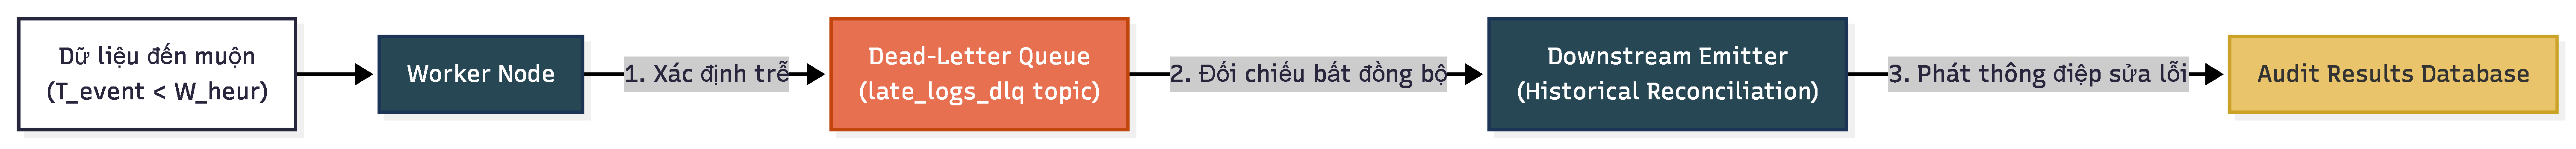
\includegraphics[width=0.9\textwidth,height=8.5cm,keepaspectratio]{Eventual_Consistency_DLQ_correction.pdf}
    \caption{Định tuyến late data sang \texttt{late\_logs\_dlq} và phát Correction Message xuống downstream (Eventual Consistency).}
    \label{fig:ddsketchdlq}
\end{figure}

\subsection{Cold Start và Conservative Prior}

Khi mới khởi động, DDSketch chưa đủ mẫu. Nếu hệ thống tin ngay vào tập mẫu nhỏ, watermark có thể tiến quá nhanh và phân loại nhầm các sự kiện hợp lệ thành late data.

Thiết kế dùng:

\begin{itemize}
    \item Warm-up phases,
    \item minimum sample count,
    \item minimum running time,
    \item Conservative Prior,
    \item baseline history.
\end{itemize}

Đây là cơ chế reliability cho approximate distributed metadata. Approximation chỉ hợp lý khi hệ thống kiểm soát giai đoạn thống kê chưa hội tụ.

\subsection{Negative Lag và Clock Skew Handling}

Hệ phân tán thường gặp \textit{clock skew}. \textit{Heuristic Watermark} xử lý rõ \textit{negative lag}:

\begin{equation}
    \ell = T_{arrival} - T_{event}
\end{equation}

Nếu \texttt{lag < 0}, hệ thống nhận diện clock skew và tránh làm nhiễm DDSketch. Điều này phù hợp với lý thuyết hệ phân tán vì không thể giả định đồng hồ vật lý giữa các sites luôn đồng bộ tuyệt đối.

\subsection{Replay-Mode Snapshot và Rollback}

Khi replay sau lỗi, các events cũ có thể tạo ra lag rất lớn. Nếu những mẫu này được đưa vào DDSketch, estimator sẽ bị nhiễm và watermark sau phục hồi sẽ sai.

Thiết kế xử lý bằng:

\begin{itemize}
    \item DDSketch snapshots,
    \item replay-mode detection,
    \item rollback về clean sketch state,
    \item tạm dừng sketch updates trong replay,
    \item recalibration khi điều kiện ổn định trở lại.
\end{itemize}

Đây là recovery protocol cho approximate metadata. Vì watermark phụ thuộc vào estimator, bảo vệ estimator trong recovery là điều bắt buộc.

\subsection{Communication Cost Trade-off}

So với \textit{Strict Watermark}, \textit{Heuristic Watermark} giảm:

\begin{itemize}
    \item phụ thuộc vào upstream Punctuation Tokens,
    \item blocking coordination,
    \item strict global proof trước khi đóng mỗi window,
    \item độ phức tạp của Coordinator.
\end{itemize}

Đổi lại, immediate consistency yếu hơn. Tuy nhiên, hệ thống bù bằng DLQ và Correction. Theo Özsu và Valduriez, đây là trade-off hợp lý khi application semantics cho phép \textit{later reconciliation}.

\subsection{Kết luận cho Heuristic Watermark}

\textit{Heuristic Watermark} được biện minh theo lý thuyết Özsu và Valduriez vì nó sử dụng:

\begin{itemize}
    \item \textit{Fragmentation} để mở rộng,
    \item \textit{Site Autonomy} để giảm latency,
    \item \textit{Distributed Processing} cho partition-local state,
    \item \textit{DDSketch} làm compact metadata estimation,
    \item lightweight global aggregation,
    \item recovery bằng snapshot và replay-mode handling,
    \item eventual correction bằng DLQ và Correction Messages.
\end{itemize}

Thiết kế này phù hợp khi \textit{low latency} và \textit{adaptive operation} quan trọng hơn \textit{Immediate Strong Consistency}.

\section{Phân tích Hệ thống dưới Định lý PACELC}

Định lý PACELC là một bản mở rộng của định lý CAP truyền thống nhằm mô tả chi tiết hơn các đánh đổi trong hệ phân tán. Định lý này phát biểu rằng: Nếu xảy ra hiện tượng phân mảnh mạng (\textbf{P}artition), hệ thống phải đánh đổi giữa tính khả dụng (\textbf{A}vailability) và tính nhất quán (\textbf{C}onsistency); ngược lại, trong điều kiện hoạt động bình thường (\textbf{E}lse), hệ thống phải đánh đổi giữa độ trễ (\textbf{L}atency) và tính nhất quán (\textbf{C}onsistency).

Hai hướng thiết kế watermark của dự án thể hiện sự lựa chọn rõ ràng trên hai góc phần tư khác nhau của định lý PACELC:

\subsection{Strict Watermark: Hệ thống PC/EC (Consistency-First)}
Strict Watermark đại diện cho mô hình thiết kế đặt tính nhất quán lên hàng đầu ở cả hai điều kiện:
\begin{itemize}
    \item \textbf{Khi xảy ra phân mảnh mạng (P $\rightarrow$ C)}: Hệ thống chọn tính nhất quán (\textbf{C}) và chấp nhận hy sinh tính khả dụng (\textbf{A}). Khi một Worker bị cô lập mạng hoặc mất kết nối, Coordinator Leader không nhận được heartbeat và tiến độ cục bộ của phân mảnh đó. Theo thuật toán tối thiểu toàn cục $W_{global} = \min(LW_i)$, hệ thống sẽ dừng tịnh tiến watermark toàn cục. Các cửa sổ xử lý ở các Worker khác bị chặn lại, không thể phát kết quả. Hệ thống chấp nhận dừng hoạt động (unavailability) để bảo đảm không phát ra dữ liệu thiếu sót.
    \item \textbf{Trong điều kiện bình thường (E $\rightarrow$ C)}: Hệ thống chọn tính nhất quán (\textbf{C}) và chấp nhận tăng độ trễ (\textbf{L}). Hệ thống thực hiện cơ chế điều phối chặn (blocking coordination), bắt buộc các Worker phải đợi Punctuation Tokens từ Ingestor và đợi tín hiệu broadcast watermark từ Coordinator Leader. Mọi cửa sổ sự kiện đều phải đợi đầy đủ bằng chứng rồi mới được chốt, khiến độ trễ đầu cuối tăng lên để đảm bảo tính đúng đắn tuyệt đối.
\end{itemize}

\subsection{Heuristic Watermark: Hệ thống PA/EL (Availability \& Latency)}
Heuristic Watermark được thiết kế nhằm tối ưu hóa hiệu năng bằng cách chấp nhận nhất quán sau cùng:
\begin{itemize}
    \item \textbf{Khi xảy ra phân mảnh mạng (P $\rightarrow$ A)}: Hệ thống chọn tính khả dụng (\textbf{A}) và chấp nhận giảm tính nhất quán (\textbf{C}). Nhờ nguyên tắc tự trị trạm (Site Autonomy), các Worker bị cô lập hoặc các Worker còn sống vẫn tiếp tục ước lượng watermark cục bộ bằng DDSketch và chốt cửa sổ để xuất kết quả ra downstream mà không bị block bởi Coordinator hay các phân mảnh bị mất kết nối.
    \item \textbf{Trong điều kiện bình thường (E $\rightarrow$ L)}: Hệ thống chọn giảm độ trễ (\textbf{L}) và chấp nhận hy sinh tính nhất quán tức thời (\textbf{C}). Dựa trên ước lượng phân vị của DDSketch, hệ thống đóng cửa sổ sớm để giảm thời gian chờ chốt. Dữ liệu đến muộn hơn watermark được chuyển hướng sang hàng đợi DLQ để sửa đổi đền bù bất đồng bộ sau (Eventual Consistency), giúp hệ thống đạt độ trễ đầu cuối cực thấp trong vận hành thực tế.
\end{itemize}

\section{So sánh hai thiết kế}

\begin{longtable}{p{0.28\textwidth} p{0.31\textwidth} p{0.31\textwidth}}
\toprule
\textbf{Khía cạnh} & \textbf{Strict Watermark} & \textbf{Heuristic Watermark} \\
\midrule
\endhead
Mục tiêu chính & Correctness và Strong Consistency & Low Latency và Adaptive Performance \\
Nguồn watermark & Punctuation Token và Local Watermarks & DDSketch Lag Estimation \\
Điều phối toàn cục & Strong Coordinator & Lightweight Aggregator \\
Consistency model & Emit khi globally safe & Emit sớm, correct sau \\
Late data handling & Cố gắng tránh late-data loss bằng cách chờ & Đưa late data vào DLQ và Correction \\
Communication cost & Cao hơn & Thấp hơn \\
Site autonomy & Thấp hơn, phụ thuộc global coordination & Cao hơn, Worker tự ước lượng cục bộ \\
Recovery model & Checkpoint, Replay, Fencing, Failback State Machine & Snapshot, Replay-Mode Rollback, DLQ Reconciliation \\
Phù hợp với & Audit, Billing, Compliance, Security & Realtime Dashboard, Monitoring, Near-Realtime Analytics \\
\bottomrule
\end{longtable}

Hai thiết kế không mâu thuẫn nhau. Chúng đại diện cho hai điểm hợp lý trong không gian thiết kế hệ phân tán:

\begin{itemize}
    \item \textit{Strict Watermark} chọn \textit{Consistency} và \textit{Reliability}.
    \item \textit{Heuristic Watermark} chọn \textit{Performance} và \textit{Autonomy}.
\end{itemize}

Lý thuyết của Özsu và Valduriez ủng hộ cả hai hướng vì hệ phân tán không tối ưu theo một chiều duy nhất. Thiết kế phải cân bằng giữa correctness, communication cost, availability, recovery và performance theo yêu cầu nghiệp vụ.

\section{Kết luận chung}

Các lựa chọn thiết kế của dự án được biện minh như sau:

\begin{enumerate}
    \item Hệ thống dùng \textit{Fragmentation} đúng cách bằng cách chia luồng log vô hạn thành Kafka partitions.
    \item Hệ thống dùng \textit{Distributed Processing} đúng cách bằng cách gán partitions cho Workers và giữ state cục bộ khi có thể.
    \item Hệ thống dùng \textit{Replication} và \textit{Checkpointing} để chịu lỗi broker, worker, coordinator và storage.
    \item Hệ thống tách rõ local metadata và global metadata thông qua local watermarks, global watermarks, DDSketch summaries và Coordinator/Aggregator state.
    \item Hệ thống xử lý recovery rõ ràng bằng Replay, Checkpoint, DLQ, Fencing Token và Failback State Machine.
    \item Hệ thống nhận thức rõ \textit{Communication Cost Trade-off} bằng cách cung cấp cả Strict path và Heuristic path.
    \item Hệ thống cung cấp \textit{Transparency} vì người dùng tương tác với một dịch vụ xử lý stream logic thống nhất dù bên trong là phân tán.
\end{enumerate}

Vì vậy, kiến trúc tổng thể tuân theo các nguyên tắc thiết kế của Özsu và Valduriez. \textit{Strict Watermark} được biện minh như một thiết kế phân tán ưu tiên \textit{Consistency}. \textit{Heuristic Watermark} được biện minh như một thiết kế phân tán ưu tiên \textit{Performance}, \textit{Autonomy} và \textit{Controlled Correction}.

\section{Tài liệu tham khảo}

Özsu, M. T., and Valduriez, P. \textit{Principles of Distributed Database Systems}. Springer.

\end{document}
